\chapter{The basics of designing, compiling and executing programming languages}

% theoretische methodischen Grundlagen, die im weiteren Verlauf bei der Problemlösung im praktischen Teil eine wichtige Rolle spielen
% Detailgrad so hoch, wie für Verständnis nötig (Leser ist anonymer Informatiker)
% >= 25%

    \section{Designing programming languages}
    
    	%TODO
    	\todo[inline]{To what degree do I need references here?}
		
		There are many different kinds of programming languages. They can vary in many aspects, from the general approach to small details. What are some important aspects?
		
		%\subsection{Domain}
		%simplicity and power
		Firstly there's the matter of what the language is trying to achieve. Is it supposed to be a generalist programming language, suitable for writing any kind of software? Or is it a domain specific language, built to solve a specific problem elegantly? In the latter case, the language will likely be a lot simpler due to its reduced scope.
		
		\subsection{Programming paradigms}
		Then there are different approaches to programming -- programming paradigms. The reader is likely familiar with imperative programming, which describes programs in terms of statements being executed to change state, and object-oriented programming, which models problems as interacting objects consisting of data and methods of working with it. Another example is functional programming, which includes no mutable state and where the results of functions are purely defined in terms of their parameters, and there are numerous other paradigms. A programming language may only follow one or be multi-paradigm, mixing them.
		
		\subsection{Type system}
		%static vs dynamic typing
		Its type system is another important aspect of a programming language, and an essential characteristic of a type system is whether it has dynamic or static typing: Values have a type, which is the set of their possible values, for example integral, boolean or array types. In static typing these types are resolved at compile time; variables and parameters have a well-defined type, either explicitly stated or inferred, and trying to use a value of incompatible type results in a compile error.
		%TODO mention how that encourages complex type systems?
		Dynamic type systems annotate values with their type at run time, and only then do type errors occur. This can make it easier to write generic code, but mistakes also go unnoticed more easily with the decrease in compile time errors.
		
		In some programming languages variables, which can usually change their value, can be marked as immutable -- or constant, as it is sometimes called in this context. The value of these variables may no longer be changed after their initial assignment. This allows for better expression of intent, preventing accidental misuse. One useful application for this is marking by-reference parameters as read-only.
		
		%TODO phrasing?
		Another concept is that of a pure function, which is one whose output depends solely on its parameters and which has no side effects. So it doesn't depend on any global state and doesn't change it. This makes it easier to reason about and test since it will always behave the same way given the same parameters. Some functional languages require all functions to be pure, while some other languages let the programmer explicitly mark the function as pure/impure, again preventing them from taking unintended actions.
		
		\subsection{Coroutines}
		
		A coroutine is a strand of execution with its own (call) stack. When the program starts, there's a single coroutine starting execution at the entry point. This coroutine may then launch new coroutines, at which point its execution is halted and the new coroutine starts its execution. They don't run in parallel, there's exactly one active coroutine (per thread) at any point. Only when this new coroutine stops its execution -- either permanently, by returning, or temporarily, by yielding; in either case a value may be passed back to the previous coroutine -- does the previous one resume its execution. A paused coroutine -- one that yielded -- may later be resumed, possibly passing in a new value.
		
		One example where coroutines are useful is iterating through recursive data structures like a binary tree. A coroutine can recurse through the tree, yielding every node it visits, which to the caller of the coroutine looks much like a function that yields the next node each time it's called.
		
		%TODO Syntax highlighting
		\begin{codelisting}[caption={Pseudocode of tree iteration using coroutines},morekeywords={function,if,for,in}]
function yield_nodes( tree ):
    if tree:
        yield tree.value
        yield_nodes( tree.left_subtree )
        yield_nodes( tree.right_subtree )

function print_nodes( tree ):
    for node in yield_nodes( tree ):
        print( node )
		\end{codelisting}
	
	\section{Compilers}
	
		%TODO
		\todo[inline]{This chapter needs references. How do I cite lectures and/or their slides, which are not publicly accessible?}
	
		Compilers translate one language -- the source language -- to another -- the target language. The Java compiler for example translates Java source code to Java Byte Code. This translation consists of multiple steps: First the input, which is essentially treated as a long sentence, is split into tokens, which can be thought of as words, by the lexer. The parser then performs a syntactical analysis on these words, creating a syntax tree. Semantic analysis then verifies this tree makes sense: Where are the referenced variables and functions? In the case of statically typed languages, do the types match? During this process, the syntax tree may be transformed and annotated with additional information. Next, optimization may take place, transforming the syntax tree into an equivalent but in some way better version, before finally the target code is generated.

		\subsection{Chomsky hierarchy}
			
			Formal languages can be derived from formal grammars, and the Chomsky hierarchy ranks these grammars by how difficult they are to parse, with Type-0 grammars being the most difficult and Type-3 grammars the easiest. Of particular interest for compiler construction are the two easiest types, Type-3 and Type-2 grammars.
			
			\subsubsection{Regular languages}
			
			Type-3 grammars describe regular languages and can be expressed as regular expressions. Regular expressions consist of terminal symbols -- characters in the alphabet of the language -- and operations combining them, as well as $\epsilon$, the empty word, which is not usually explicitly used outside of formal definitions but implied in absence of a character. These are the core operations:
			
			 %The first operation is concatenation, and is simply written as such: $ab$ means expression $a$ followed by expression $b$. The alternative operator $|$ is usually understood to have a lower precedence than concatenation, so $ab|cd$ means $(ab)|(cd)$ and explicit parentheses are required if the intended meaning is $a(b|c)d$. The operation with the highest precedence is the unary Kleene star, which is defined as any number of concatenations, including none, i.e. the empty word; it's written as $a*$, which 
			
			\begin{center}
			\begin{tabular}{ l l p{10cm} }
			\toprule
			Name         & Syntax & Description \\
			\midrule
			Concatenation & \lstinline$ab$  & Expression \lstinline$a$ followed by expression \lstinline$b$. \\
			Alternative   & \lstinline$a|b$ & Either expression \lstinline$a$ or expression \lstinline$b$; lower precedence than concatenation, so \lstinline$ab|cd$ means \lstinline$(ab)|(cd)$ and explicit parentheses are required if \lstinline$a(b|c)d$ is the intention. \\
			Kleene Star   & \lstinline$a*$  & Any number of repetitions of expression \lstinline$a$, including none, i.e. $\epsilon$\lstinline$|a|aa|aaa|$$\ldots$; highest precedence, so \lstinline$ab*c$ means \lstinline$a(b*)c$. \\
			\bottomrule
			\end{tabular}
			\end{center}
			
			Some auxiliary operators are often defined in terms of them, like \lstinline$a+ = aa*$ and \lstinline$a? = a|$$\epsilon$, but those are merely substitutions, they don't add any capabilities, and thus don't require further investigation. Other useful shorthands are bracket expressions like \lstinline$[a-d0-3_] = a|b|c|d|0|1|2|3|_$, which allow for the compact definition of large alternatives, the dot (\lstinline$.$), which matches any one character, and \lstinline$[^a-c]$, which matches any one character except \lstinline$[a-c]$.
			
			Regular languages can be recognized by finite automatons in $\mathcal{O}(n)$ time where $n$ is the length of the input. That's as good as it gets with linear input: Each character has to be processed. So how does a finite automaton work?
			
			\todo[inline]{Do I need to use mathematical notations? I find precisely worded sentences to be easier to understand and write.}
			
			There are two kinds of finite automatons: deterministic and non-deterministic finite automatons. The more practical one to build is the deterministic finite automaton (DFA). It has a finite set of states, one of which is the start state and some of which are accept states; an input alphabet; and a transition function which defines the resulting state for a given current state and input character. Initially, the automaton is in its start state; the input is then processed one character at a time: the current state changes according to the transition function given the current input character, until all input characters have been processed and a certain state has been reached. If this state is an accept state, the input is accepted, i.e. it is part of the regular language.
			
			The transition function can be partial; if it is not defined for a given state-character-pair, the input is not accepted. This simplifies its definition. If a total definition is preferred, a fail-state to which all formerly undefined transitions lead can be introduced.
			
			Non-deterministic finite automatons (NFAs) are mostly the same, only the transition function works differently: Firstly, it does not define a single resulting state for any given input, but a set of possible resulting states, any of which may be entered. Secondly, it is not just defined for input characters, but also $\epsilon$ inputs, i.e. spontaneous $\epsilon$-transitions that consume no input are possible. An input is thus considered accepted if its processing \textit{may} end in an accept state. Due to their non-deterministic nature DFAs are impractical to build, but as an intermediate model they are useful, as will become apparent shortly.
			
			Finite automatons can be represented as directed graphs, with states being the nodes and transitions being the edges, annotated with the input. By convention, accept states are encircled and the start state is indicated by an arrow pointing to it. This notation will be used frequently throughout this chapter due to its simplicity and brevity.
			
			NFAs are so useful in the context of compilers because regular expressions can be directly translated to them. Only a handful of rules have to be applied recursively, as outlined in figures \ref{fig:re_nfa_char}--\ref{fig:re_nfa_kleene}\footnote{To understand the need for states 1 and 4 in figure \ref{fig:re_nfa_kleene} think about the translation of \lstinline$a*b*$.}. A simple example of this is given in figure \ref{fig:re_nfa_example}.
			
			
			\begin{figure}
			\centering
			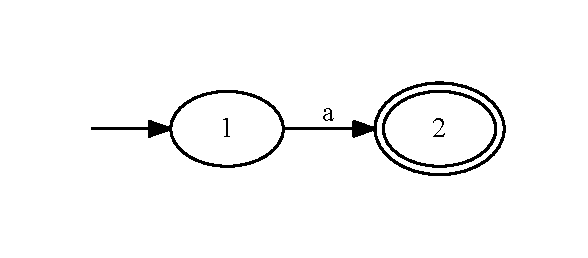
\includegraphics{figures/re_char}
			\caption{NFA for the regular expression ``\lstinline$a$'' -- i.e. a single character}
			\label{fig:re_nfa_char}
			\end{figure}
			
			\begin{figure}
			\centering
			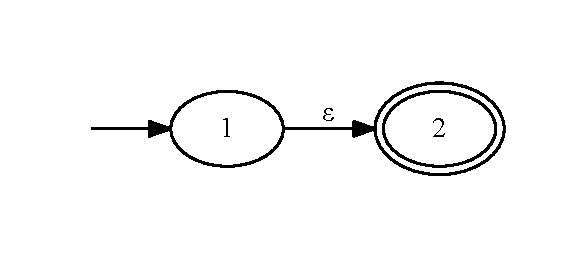
\includegraphics{figures/re_epsilon}
			\caption{NFA for the regular expression ``'' -- i.e. the empty string}
			\label{fig:re_nfa_epsilon}
			\end{figure}
			
			\begin{figure}
			\centering
			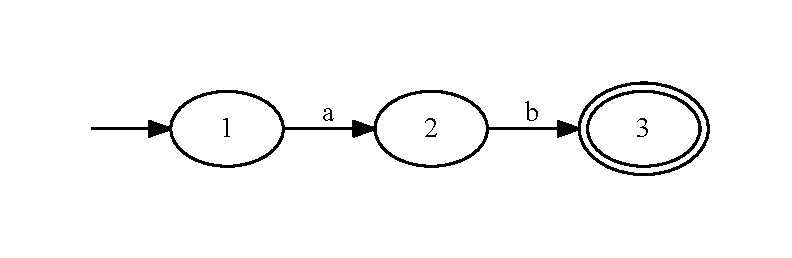
\includegraphics{figures/re_sequence}
			\caption{NFA for the regular expression ``\lstinline$ab$'' -- i.e. a concatenation}
			\label{fig:re_nfa_concatenation}
			\end{figure}
			
			\begin{figure}
			\centering
			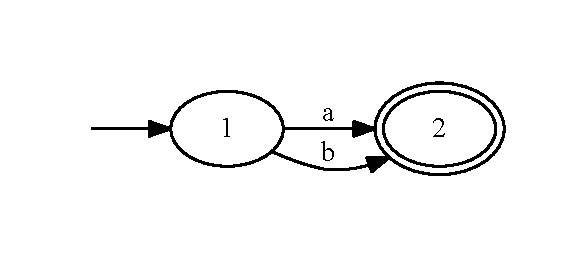
\includegraphics{figures/re_alternative}
			\caption{NFA for the regular expression ``\lstinline$a|b$'' -- i.e. an alternative}
			\label{fig:re_nfa_alternative}
			\end{figure}
			
			\begin{figure}
			\centering
			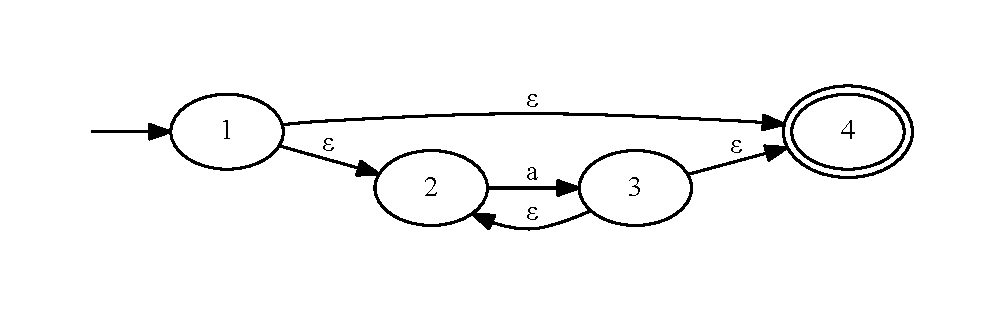
\includegraphics[width=\textwidth]{figures/re_kleene}
			\caption{NFA for the regular expression ``\lstinline$a*$'' -- i.e. a repetition}
			\label{fig:re_nfa_kleene}
			\end{figure}
			
			\begin{figure}
			\centering
			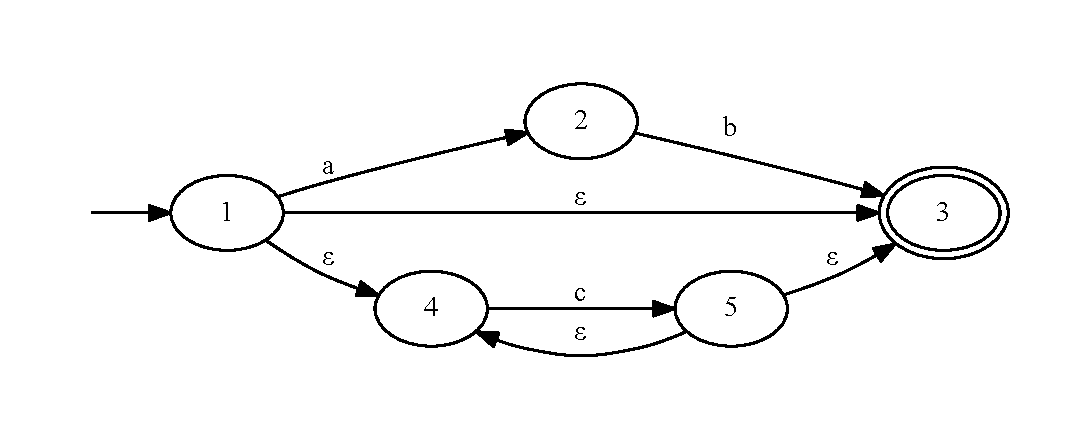
\includegraphics[width=\textwidth]{figures/re_example}
			\caption{NFA for the regular expression ``\lstinline$ab|c*$''}
			\label{fig:re_nfa_example}
			\end{figure}
			
			NFAs may be impractical to build, but any NFA can be converted into a (practical) DFA accepting the same language. This DFA has as its states sets of states from the NFA: The initial state is the set containing the NFA's initial state and any state reachable from it using $\epsilon$-transitions. For each character there's a transition to the set of NFA states reachable from any of the states in the previous set using this character and any number of $\epsilon$-transitions. Accept states are all sets containing NFA accept states.
			
			By way of an example, figure \ref{fig:re_dfa_example} shows the DFA equivalent of the NFA in figure \ref{fig:re_nfa_example}, constructed according to these rules.
			
			\begin{figure}
			\centering
			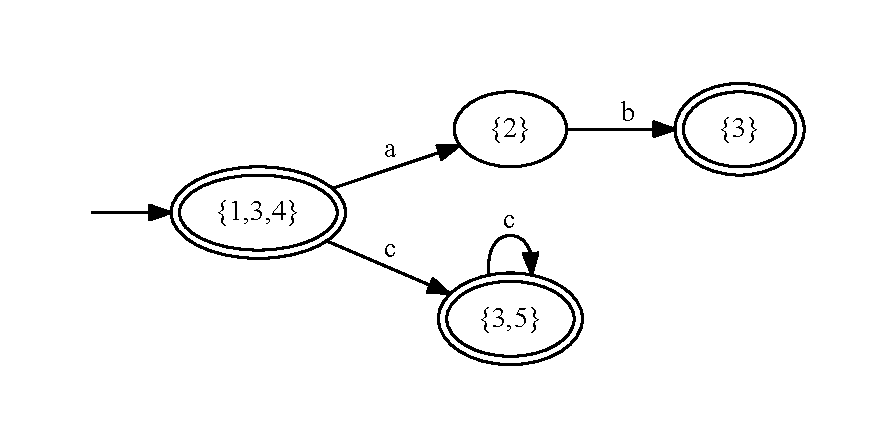
\includegraphics[width=\textwidth]{figures/re_example_dfa}
			\caption{DFA equivalent of the NFA in figure \ref{fig:re_nfa_example}}
			\label{fig:re_dfa_example}
			\end{figure}
			
			Large DFAs can often be simplified, eventually resulting in a minimal DFA. One way of finding it is the table-filling algorithm, in which equivalent states are determined and merged: Any two states are distinguishable if one of them is an accept state and the other one is not, so that is the initial set of demonstrably different state pairs. An any two states that given the same input transition into distinguishable states are also distinguishable, so those are added to the set as well. This is repeated until a fixed point is found, i.e. until no more distinguishable pairs are found. All the remaining pairs are equivalent and can be merged without affecting the language accepted by the DFA. Assuming there are no unreachable states, which should have already been eliminated during the transformation from NFA to DFA, this is now the minimal DFA.
			
			%TODO
			\todo[inline]{Do I need some kind of conclusion here?}
			
			\subsubsection{Context-free languages}
			
			Regular expressions have the aforementioned desirable property of processing input in $\mathcal{O}(n)$ time; but they are limited in the kinds of languages they can express. In particular, they lack recursion, which prevents them from expressing matching parentheses, for example; that's where Type-2 grammars come into play.
			
			Type-2 grammars describe context-free languages and are primarily defined by their productions, which are substitution rules that define how to derive valid words of the language from a start symbol. More specifically, a context-free grammar is defined by: Its terminal symbols, i.e. the alphabet of the language described by it; its non-terminal symbols, i.e. substitution placeholders in terms of which the language is defined, one of which is the start symbol; and the productions, which are the substitution rules of the non-terminal symbols.
			
			A production maps a non-terminal symbol to a sequence of terminal and non-terminal symbols; possibly to $\epsilon$, the empty sequence. Here's a an example of the productions for a grammar describing sum expressions, with the terminal symbols ``+'' and ``number'' and the non-terminal symbol Expression, which is also the start symbol:
			
			Expression $\rightarrow$ Expression ``+'' Expression\\
			Expression $\rightarrow$ ``number''
			
			Words can be derived by repeatedly applying these productions until only terminal symbols remain. This process can be visualized using trees; figure \ref{fig:derivation_tree_exp_1} shows a possible derivation yielding ``number+number+number.'' The inner nodes are the non-terminal symbols, the leafs the terminal symbols; concatenating the leafs in order yields the word.
			
			\begin{figure}
			\centering
			\begin{forest}
			[Expression
				[Expression
					[``number'']
				]
				[``+'']
				[Expression
					[Expression
						[``number'']
					]
					[``+'']
					[Expression
						[``number'']
					]
				]
			]
			\end{forest}
			\caption{Deriving ``number+number+number''}
			\label{fig:derivation_tree_exp_1}
			\end{figure}
			
			However that's not the only way to derive ``number+number+number'' using those productions; figure \ref{fig:derivation_tree_exp_2} shows a different way. There are multiple ways of deriving the same word -- the grammar is ambiguous. Some context free grammars are inherently ambiguous, but often ambiguous grammars can be transformed into non-ambiguous grammars corresponding to the same language.
			
			\begin{figure}
			\centering
			\begin{forest}
			[Expression
				[Expression
					[Expression
						[``number'']
					]
					[``+'']
					[Expression
						[``number'']
					]
				]
				[``+'']
				[Expression
					[``number'']
				]
			]
			\end{forest}
			\caption{Deriving ``number+number+number'' a different way}
			\label{fig:derivation_tree_exp_2}
			\end{figure}
			
			A non-ambiguous version of the sum expression grammar above could have these productions:
			
			Expression $\rightarrow$ Expression ``+'' ``number''\\
			Expression $\rightarrow$ ``number''
			
			This grammar has what is called a left-recursion: The right side of the first Expression production starts with Expression. This is of interest when generating parsers and will be brought up again later. The resulting derivation tree is shown in figure \ref{fig:derivation_tree_exp_3} -- note how the left-recursion results in it growing towards the left.
			
			\begin{figure}
			\centering
			\begin{forest}
			[Expression
				[Expression
					[Expression
						[``number'']
					]
					[``+'']
					[``number'']
				]
				[``+'']
				[``number'']
			]
			\end{forest}
			\caption{Deriving ``number+number+number'' using an unambiguous grammar}
			\label{fig:derivation_tree_exp_3}
			\end{figure}
			
			\todo[inline]{This is a very abrupt end?}
		
		\subsection{Lexer}
		
			In the interest of simplifying the file to be compiled it is usually first split into logical pieces called tokens; for example numbers, comments, operators, whitespace or identifiers. This so-called lexical analysis is done by a lexer, also known as a scanner or tokenizer.
			
			The tokens are defined through regular expressions; they are ranked, usually implicitly by order of definition; and then the longest prefix match of the input is consumed, breaking ties using the ranking. This yields a single token, which is annotated with the input it matched in case that is later needed. (Take for example a ``number'' token, which uses the regular expression \lstinline$[0-9]+$: in order to be able to tell which number was matched, the matched string is required.) Then, a new token is consumed from the remaining input and so on until none is left or until there is no match, in which case the input is invalid.
			
			This is achieved by determining the NFAs corresponding to the tokens' regular expressions, annotating their accept states with the corresponding token names and merging them by creating a new initial state with $\epsilon$-transitions to all their (former) initial states. The result is an NFA accepting all tokens, which is then converted to a DFA and minimized. During minimization accept states annotated with different tokens may be merged; in this case the token with the highest ranking is kept.
			
			The lexer then stores the input location when the DFA was last in an accept state, as well as the corresponding token. When the DFA reaches an invalid state (i.e. the transition function is undefined for the current character, if it is partial, or an explicit fail-state is entered) or the end of input, the lexer goes back to this location and emits or ignores the stored token. The DFA is then reset to its initial state the next token is parsed. Due to this backtracking the time complexity is no longer $\mathcal{O}(n)$; in the worst case it is $\mathcal{O}(n^2)$, but given typical token definitions and inputs it will usually still be close to $\mathcal{O}(n)$.
			
			Undesired tokens can be filtered at this point; whitespace and comments are usually irrelevant, for example, and can be omitted from the output, potentially simplifying the grammar significantly.
		
		\subsection{Parser}
			
			Next is the syntactical analysis or parsing, which aims to turn the tokens into a syntax tree according to the language's grammar. The syntax is typically defined in terms of an unambiguous context-free grammar and the challenge is to create an efficient parser based on that.
			
			\subsubsection{LL Grammars}
			
			One approach to parsing is using recursive descent, which starts with the start symbol, the root of the syntax tree, and recursively builds it top-down. In this case there is a parsing function for each symbol and applying a production translates to sequentially calling all the according symbol functions.
			
			So when there are multiple productions for a given non-terminal symbol, which one is chosen? In LL($k$) parsing the production is chosen based on the next $k$ tokens; to this end a table is calculated, with the row corresponding to the non-terminal symbol being parsed and each column a $k$-token sequence; the cells contain the production to be used under those conditions. Since the number of $k$-token sequences grows exponentially, $k$ is usually just $1$, i.e. the production is chosen based on the next token.
			
			That's one reason why using a lexer is useful: Knowing that the next character is ``i'' is much less useful than knowing the next token is ``if.''
			
			For many grammars the choice of production is ambiguous. Grammars in which it is not are called LL($k$) grammars, and many context-free grammars can be transformed into LL($k$) grammars. One property that keeps grammars from being LL($k$) is containing left-recursions, in which case the depth of the recursion can't be determined from the first $k$ tokens. this can be fixed by transforming the grammar into a right-recursive one, although this changes the semantic: Left-associative operators become right-associative, \lstinline$a-b-c$ is interpreted as \lstinline$a-(b-c)$ instead of \lstinline$(a-b)-c$. If this is undesirable, a post processing step is required.
			
			\subsubsection{LR Grammars}
			
			A different approach, LR parsing, is similar to LL parsing in a lot of ways. It's also a predictive parser for a certain class of context-free grammars that determines the next step based on $k$ tokens lookahead (also typically 1) based on a parse table. However, unlike LL, it doesn't work top-down, starting with the root of the parse tree and expanding the left-most non-terminal symbol, it's a bottom-up parser starting at the leafs, the terminal symbols, combining them into non-terminal symbols as it goes along.
			
			To this end processed terminals and non-terminals are kept on a stack and the decision to be made is whether to shift -- i.e. read and push the next terminal symbol onto the stack -- or reduce -- i.e. combine the symbols on the top of the stack into a non-terminal symbol. As with the LL parser this decision is made based on the next token(s).
			
			And just like LL parsing LR parsing needs a certain type of grammar to be able to unambiguously determine the next action, an LR grammar. Each LL grammar can be converted to an LR grammar, but some LR grammars have no LL equivalent.
			
			LR parsing, like LL parsing, by virtue of making a final parse decision is $\mathcal{O}(n)$.
			
			\subsubsection{Parsing Expression Grammars}
			
			Parsing expression grammars (PEGs) are an alternative to context-free grammars for defining syntax\cite{peg}. While context-free grammars describe how to generate a language, PEGs describe how to parse a language into a syntax tree. To this end they use the following operators:
			
			\begin{center}
			\begin{tabular}{ l l p{10cm} }
			\toprule
			Name               & Syntax          & Description \\
			\midrule
			Sequence           & \lstinline$ab$  & Expression \lstinline$a$ followed by expression \lstinline$b$. \\
			Prioritized Choice & \lstinline$a/b$ & If it parses, \lstinline$a$; (only) if it doesn't, \lstinline$b$. \\
			Zero-or-more       & \lstinline$a*$  & Greedily parse as many \lstinline$a$ as possible. \\
			One-or-more        & \lstinline$a+$  & Greedily parse as many \lstinline$a$ as possible, at least one. \\
			Optional           & \lstinline$a?$  & If it parses, \lstinline$a$. \\
			And-predicate      & \lstinline$&a$  & Match \lstinline$a$, then backtrack, i.e. fail if \lstinline$a$ does not match, but don't consume it if it does. \\
			Not-predicate      & \lstinline$!a$  & Like \lstinline$&a$, but fail if and only if \lstinline$a$ matches. \\
			\bottomrule
			\end{tabular}
			\end{center}
			
			Some of these operators (\lstinline$*$, \lstinline$+$ and \lstinline$?$) are reminiscent of regular expressions; but unlike their regular expression counterparts, they are not non-deterministic but greedy, i.e. they will match as much as possible. This, along with the prioritized choice, makes PEGs inherently unambiguous.
			
			A typical example of ambiguous context-free grammars is the dangling else: In if-statements with an optional else, nesting can lead to ambiguity: \lstinline$if(x) if(y) a() else b()$ could be parsed as \lstinline$if(x){ if(y) a() else b() }$ or \lstinline$if(x){ if(y) a() } else b()$, but with a greedy optional operator it will always parse as the former.
			
			Like LL grammars, PEGs can be parsed using recursive descent. Instead of predicting which branches to take as with LL grammars, multiple may be tried and subsequently discarded until a match is found. This backtracking can lead to exponential runtime, but that can be avoided: The packrat algorithm\cite{packrat} allows for parsing PEGs in $\mathcal{O}(n)$ through the use of memoization. However the overhead introduced by memoization may still make this slower than a naive backtracking algorithm in practice in a given implementation for typical inputs; few practical PEG implementations use packrat parsers.
			
		\subsection{Semantic Analysis}
		
		Once the source code has been parsed into a syntax tree, further analysis calculates node attributes and possibly transforms it. Nodes might need to be rearranged to achieve left-associative operators in the case of a grammar free of left-recursions, for example.
		
		Unlike the parser, the semantic analysis is not context-free: During the traversal of the tree information can be collected for later use. For example this usually includes variables: They typically need to be defined first and can from then on be referred to within the same scope. This is also where it can be ensured that immutable variables aren't changed. And in statically typed languages this is where type checks happen; to this end all (sub-)expressions can be annotated with their type. And this is also where function calls are usually resolved, possibly determining which overload to call based on the calculated argument types.
		
		Since the semantics of different languages vary, so does their semantic analysis. What exactly happens at this point is largely up to the language designer.
		
		%register allocation?
		
		\subsection{Code generation}
		
		Finally, the machine code to be executed is generated based on the annotated syntax tree. How exactly this happens largely depends on the machine being targeted and there may actually be multiple code generators for different targets if the code is supposed to run on various machines.
		
		When generating code for a register-based machine (which will be further examined in the section on virtual machines), one part of the process is register allocation: It has to be determined which values are stored in which register, since their number may be limited. On a stack-based machine, on the other hand, all values are kept on a stack and register allocation is not required.
		
		The code may also be subject to further optimization: It may be possible to determine that some code will never be executed -- this so called ``dead code'' may be removed; tail call optimization can turn function calls at the end of a function into unconditional jumps, keeping the call stack smaller; and various other techniques.

	\section{Virtual Machines}
	
		Compilers can target actual processors and generate native machine code for them to execute, and that is the fastest method since there are no additional abstraction layers; but sometimes it is desirable to run the code on a simulated computer in a so-called virtual machine, or VM for short. This can be for security reasons -- a VM can be ``sandboxed,'' preventing code executed in it from accessing other parts of the host system; because a machine with different properties than the host machine is desired; to have a unified execution environment across different types of machines; or for various other reasons.
		
		As the name implies a virtual machine simulates an actual machine; so it typically repeatedly fetches an instruction from the machine code and executes it. The Instruction Pointer (IP) keeps track of the current location in the code and automatically increments past the current instruction upon fetching it. An instruction consists of an opcode (short for operation code) defining the operation to be performed and possibly various operands, if the operation calls for them; the exact encoding of these is machine-specific.
		
		Common instructions include various kinds of jumps and calls that move the instruction pointer, allowing for loops and branches in the execution; instructions for reading from and writing to memory; arithmetic instructions for integer and floating point calculations; and boolean operations. Additional instructions are included as necessary.
		
		To realize function calls, a call stack is used. It is used to pass parameters to functions and store local variables -- these vary between calls, and since functions can be called recursively there may be multiple calls to a function simultaneously, hence a stack. It is also used to store the return address: upon calling a function, the address where execution is to be resumed upon return from the function is stored on the stack in addition to the parameters. The sum of this per-call data -- parameters, local variables and return address -- is called a stack frame; it can either just be an implicit interpretation of the data on the stack or an explicit data structure stored on the stack.
		
		Intermediate results of the evaluation of expressions can also be stored on a stack -- the top values are then implicitly the operands for arithmetic instructions. So to calculate \lstinline$2+(x*3)$ the code first pushes \lstinline$2$ onto the stack, then the value of \lstinline$x$, finally \lstinline$3$ before first doing a multiplication and then an addition.
		
		The alternative to using such an evaluation stack is the usage of registers to store values; in this case the aforementioned register allocation is required. Here the machine has a number of registers and an instruction explicitly names the operand and target registers. This is similar to how many real machines, such as x86 processors, work and thus simplifies Just-In-Time (JIT) compilation, which is the translation of parts of the VM byte code that have been determined to be performance critical to native machine code at run time.
		
		Coroutines require explicit support in the VM -- they essentially need their own call stack and instruction pointer (and possibly evaluation stack or registers), and there need to be instructions to create, pause and resume them.
		
		VMs also have the option of managing their memory differently; instead of making heap allocations and manually freeing them later, they can use garbage collection. There are various types of garbage collection, but the general idea is to check for memory that is no longer in use, usually periodically; to this end the VM needs to be able to interpret the memory and recognize pointers. Garbage collection relieves the programmer of memory management but introduces overhead; periodic garbage collection can take significant time, resulting in brief unresponsiveness when it runs.
		
		For a program to be able to cleanly shut down in case of an error the VM also needs to be capable of stack unwinding, which is the proper cleanup of stack frames e.g. due to an exception. This may include running the destructors\footnote{In certain object-oriented programming languages a class may define a special destructor method to be run when an object is destroyed, which usually takes care of cleaning up resources.} of local objects, special deferred cleanup statements\footnote{Some languages have a \lstinline$defer$ keyword to define statements to be executed once the current scope is left.} or similar. This too requires the VM to be aware of the types of values on the stack.
	
	\section{Relevant software patterns and language features}
		
		A grasp of a couple of concepts is required for understanding the coming chapters; these are explained in this section.		
		%TODO why C++14?
		
		\subsection{Resource Acquisition Is Initialization (RAII)}
		
		RAII is the idea that object lifetime should represent resource lifetime. Resources are acquired during object construction and released upon destruction.
		
		Take for example C++'s string class, \lstinline$std::string$. In its constructor it allocates the memory required to hold its content, in its destructor the memory is freed. Since stack unwinding ensures the destructor will be called upon object destruction, memory leaks are impossible.
		
		Closely related to this are move mechanics: Resources can be moved from one object into another if they no longer need to be available in the original object. To this end C++ allows for the explicit definition of move constructors -- for constructing a new object by moving the resources of another into it -- and move assignment -- for moving the contents of one existing object into another. Moving is usually preferable to copying since it's faster, but occasionally a copy is desired.
		
		\subsection{Type Parameters}
		
		C++ allows to parameterize functions or classes with types using templates. This allows you to define e.g. a set of elements of a given type, as long as comparison for elements of that type is defined, using \lstinline$std::set<T>$, where \lstinline$T$ is the type of choice. It's also possible to define types with an arbitrary number of template parameters, for example a tuple, in which case algorithms are defined recursively.
		%TODO elaborate?
		
		\subsection{Function Overloading}
		
		Function overloading allows multiple functions may have the same name as long as their parameters vary in type. The function to call is then determined based on the type of the supplied parameters. C++ also allows for the overloading of operators, allowing programmers to define e.g. \lstinline$+$ for their own types.
		
		\subsection{Sum Types}
		
		A sum type is much like a union in C in that in can hold different types, except it knows which one it currently holds. \lstinline$boost::variant$ is one C++ implementation of a sum type which also supports recursive variants.
		%TODO elaborate?
		
		\lstinline$boost::variant$ allows for the selection of how to handle a given variant object through the use of a visitor object which defines different overloads of a function for each possible variant type, of which the one corresponding to the actual type of the variant is then called.
		
		\subsection{Optional Types}
		
		\lstinline$boost::optional$ represents a value that may be omitted. In this it is much like a null-pointer, which allows for omission of a valid pointer, but without requiring the use of pointers and the dynamic memory usage that may come with it.
		
		\subsection{Iterators}
		
		Traversal of containers in C++ is usually done using iterators, which hide the implementation details of the container from the user, who just get an interface for moving through the elements in the container and accessing them. Depending on the kind of object being traversed, iterators may just be able to move forwards in single step increments, or may also be able to move backwards or by a certain distance, and may or may not be copyable.
		
		Depending on the container, certain operations may invalidate iterators; always the deletion of the element it points to, for example, and usually the relocation of elements as well.
		
		\subsection{Serialization}
		
		The act of transforming an object into a stream of bytes representing it is called serialization. The inverse act of recreating the object is called de-serialization. They are commonly used to save objects to a file or send them over a network.
		
		How and if an object is serialized varies. It's analogous to copying in a lot of ways, and like the differentiation into deep and shallow copies nested objects can either be serialized as well or just stored as some kind of reference which is then looked up during de-serialization. And since it's essentially a form of copying the object, uncopyable objects can't be serialized either; like for example file handles.
